\documentclass[letterpaper,10pt]{article}

\usepackage{enumitem}
\usepackage{titling}
\usepackage{listings,listings-rust}
\usepackage{url}
\usepackage{soul}
\usepackage{hyperref}
\usepackage{setspace}
\usepackage{subfig}
\usepackage{sectsty}
\usepackage{pdfpages}
\usepackage{colortbl}
\usepackage{multirow}
\usepackage{multicol}
\usepackage{relsize}
\usepackage{amsmath}
\usepackage{wasysym}
\usepackage{fancyvrb}
\usepackage[yyyymmdd]{datetime}
\usepackage{amsmath,amssymb,amsthm,graphicx,xspace}
\usepackage[titlenotnumbered,noend,noline]{algorithm2e}
\usepackage[compact]{titlesec}
\usepackage{XCharter}
\usepackage[T1]{fontenc}
\usepackage[scaled]{beramono}
\usepackage[normalem]{ulem}
\usepackage{booktabs}
\usepackage{tikz}
\usetikzlibrary{arrows.meta,automata,shapes,trees,matrix,chains,scopes,positioning,calc,decorations.pathreplacing}
\tikzstyle{block} = [rectangle, draw, fill=blue!20, 
    text width=2.5em, text centered, rounded corners, minimum height=2em]
\tikzstyle{bw} = [rectangle, draw, fill=blue!20, 
    text width=4em, text centered, rounded corners, minimum height=2em]

\definecolor{namerow}{cmyk}{.40,.40,.40,.40}
\definecolor{namecol}{cmyk}{.40,.40,.40,.40}
\renewcommand{\dateseparator}{-}

\let\LaTeXtitle\title
\renewcommand{\title}[1]{\LaTeXtitle{\textsf{#1}}}

\lstset{basicstyle=\footnotesize\ttfamily,breaklines=true}

\newcommand{\CPP}{C\nolinebreak\hspace{-.05em}\raisebox{.4ex}{\tiny\bf +}\nolinebreak\hspace{-.10em}\raisebox{.4ex}{\tiny\bf +}}
\def\CPP{{C\nolinebreak[4]\hspace{-.05em}\raisebox{.4ex}{\tiny\bf ++}}}

\newcommand{\handout}[5]{
  \noindent
  \begin{center}
  \framebox{
    \vbox{
      \hbox to 5.78in { {\bf ECE459: Programming for Performance } \hfill #2 }
      \vspace{4mm}
      \hbox to 5.78in { {\Large \hfill #4  \hfill} }
      \vspace{2mm}
      \hbox to 5.78in { {\em #3 \hfill \today} }
    }
  }
  \end{center}
  \vspace*{4mm}
}

\newcommand{\lecture}[3]{\handout{#1}{#2}{#3}{Lecture#1}}
\newcommand{\tuple}[1]{\ensuremath{\left\langle #1 \right\rangle}\xspace}

\addtolength{\oddsidemargin}{-1.000in}
\addtolength{\evensidemargin}{-0.500in}
\addtolength{\textwidth}{2.0in}
\addtolength{\topmargin}{-1.000in}
\addtolength{\textheight}{1.75in}
\addtolength{\parskip}{\baselineskip}
\setlength{\parindent}{0in}
\renewcommand{\baselinestretch}{1.5}
\newcommand{\term}{Winter 2020}

\singlespace


\begin{document}

\lecture{ 37 --- Ownership in Rust }{\term}{Patrick Lam}

\paragraph{Runtime safety.} We said that Rust is safe. One way in which it is safe is for
arrays. Rust has tuples and structs. Hard to go out of bounds on those. Rust also has arrays.
Like with any language, one can imagine going beyond the ends of an array. Rust defines
the behaviour of going beyond the end of an array: it is a runtime exception (``panic''),
unlike C/C++, where it is undefined behaviour.

\vspace*{-2em}
\begin{lstlisting}[language=Rust]
  let a = [1,2,3,4,5];
  let index = 10;
  println!("error! {}", a[index]); // panics here.
\end{lstlisting}

\subsection*{What's special about Rust?}
Let's step back and do some Rust propaganda.
\begin{itemize}[noitemsep]
\item harder to write unsafe code: compiler + runtime ensure safety. No arrays-out-of-bounds accesses, null pointers (at all), wild pointers;
\item yet can still write low-level code;
\item supports zero-cost abstractions (like C++ as discussed in L18);
\item designed with ergonomics in mind;
\item type system obviates need for either garbage collection or manual memory management (which you will get wrong)\footnote{Well, mostly. Sometimes you need to use ref-counted data, and we'll see that.};
\item type system prevents race conditions;
\item dependency management using crates.
\end{itemize}
As far as I know, Firefox's rendering engine, Project Servo, is the largest deployed Rust codebase. [size?]

\paragraph{Rust lectures outline.} Here's what else we are going to talk about. Chapter references from
\emph{The Rust Programming Language}.
\begin{enumerate}[noitemsep]
\item[Ch4:] what's special about Rust: \emph{ownership};
\item[Ch15:] smart pointers (briefly);
\item[Ch16:] fearless concurrency.
\end{enumerate}
Also relevant to this course, but here we are in week 12, so we're not going to talk about it.
\begin{enumerate}[noitemsep]
\item[Ch10:] lifetimes;
\item[Ch19:] unsafe Rust.
\end{enumerate}

\section*{Ownership in Rust [Chapter 4.1]}
Also known as ``how to fight the borrow checker and win''.

Rust uses ownership types to manage its heap. Ownership types were not invented by the Rust
community, but Rust is the first production-scale language to deploy it. The alternatives
are {\tt malloc}/{\tt free} in C, or {\tt new}/GC in Java. Rust does still have a stack, but
we'll see when things go on the stack vs when they go on the heap.

\subsection*{The Rules}
\begin{enumerate}[noitemsep]
\item Each value in Rust has a variable that \emph{owns} it.
\item This variable is \emph{unique}.
\item When the owner goes out of scope, the value will be dropped (aka freed).
\end{enumerate}

Variable scopes are fairly standard.
\begin{lstlisting}[language=Rust]
  fn main() {
    println!("start");
    { // no s
      let s = "I am s";
      println!("s is {}", s);
    } // s now out of scope
  }
\end{lstlisting}

OK, let's put something on the heap. We'll be using Rust {\tt String} objects rather than
string literals. String literals are compile-time constants. String objects contain a heap component,
which may be allocated and freed.

(What can go wrong with heap allocation? You might not free/free too late;
free too early; double free. GC manages this through an approximation: if you have no more pointers to it,
then it doesn't spark joy, and you don't need it anymore. Rust goes a different way.)
\begin{lstlisting}[language=Rust]
  fn main() {
    let s = String::from("hello"); // immutable String
    let mut s2 = String::from("459 assignments"); // mutable String
    s2.push_str(", maybe?");
    println!("got string {}", s);
  }
\end{lstlisting}

Rust uses rule \#3: if something goes out of scope, then drop (free) it.
This is quite like C++ RAII (Resource Acquisition is Initialization).

Still, we need a solution for objects that live beyond their original scope, e.g.
return values.
\begin{lstlisting}[language=Rust]
  fn return_a_string() -> String {
    let s = String::from("longevity");
    return s; // transfers ownership (moves) to caller
  }

  fn main() {
    let returned_string = return_a_string();
    println!("string {}", returned_string);
  }
\end{lstlisting}

So, Rust frees owned values when variables go out of scope. Also, Rust calls
``drop'' (akin to a destructor) on objects that go out of scope. Note that
going out of scope, not the drop call, is what actually causes the free.

\section*{Transferring Ownership (aka move semantics)}

Let's look at an example.
\begin{lstlisting}[language=Rust]
  let s1 = String::from("no surprise");
  println!("can print {}", s1);
  let s2 = s1;
  println!("can still print {}", s2);
  println!("this line won't compile! {}", s1); // no longer owns
\end{lstlisting}

(Note that string literals, or ints, or anything only on the stack,
doesn't have this behaviour---they are copied, or technically, they
have the ``Copy'' trait.)

OK, so what's going on? Let's take a step back.

Rust strings are a hybrid, containing both a stack part and a heap part.

\begin{center}
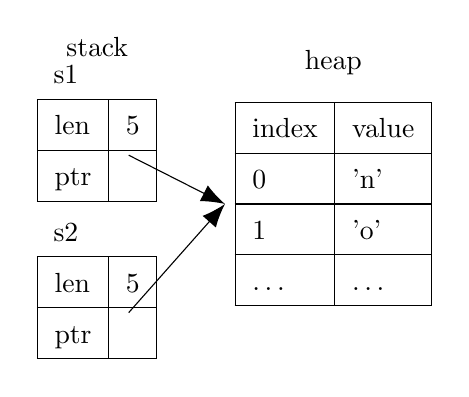
\begin{tikzpicture}
\draw (0,1) node {stack};
\draw (0,0) node (one) {
\begin{tabular}{|l|l|}
\multicolumn{2}{l}{s1} \\
\hline
len & 5 \\ \hline
ptr & \\ \hline
\end{tabular}
};

\draw (0,-2) node (two) {
\begin{tabular}{|l|l|} 
\multicolumn{2}{l}{s2} \\ \hline
len & 5 \\ \hline
ptr & \\ \hline
\end{tabular}
};

\draw (3,0.8) node {heap};
\draw (3, -1) node (s) {
\begin{tabular}{|l|l|} \hline
index & value \\ \hline
0 & 'n' \\ \hline
1 & 'o' \\ \hline
\ldots & \ldots \\ \hline
\end{tabular}
};

\path[draw,-{Latex[length=3mm]}] (one) ++ (0.4,-0.38) -- (s.west);
\path[draw,-{Latex[length=3mm]}] (two) ++ (0.4,-0.38) -- (s.west);

\end{tikzpicture}
\end{center}

The assignment {\tt let s2 = s1} carries out a shallow copy of the stack part. Rust
does not automatically copy the heap part.

Now, recall that Rust has automatic memory reclamation. How can that
work? What gets freed?  Here, {\tt s1} and {\tt s2} are in the same
scope. When they go out of scope, what should get freed? We
don't want to double free.

\paragraph{Key idea.} For automatic memory reclamation to work, we give {\tt let s2 = s1} \emph{move semantics}
(as in C++). After the move, {\tt s1} is no longer valid.
Ownership of the heap part is moved from {\tt s1} to {\tt s2} by the assignment.

That is, {\tt s1} no longer owns the heap object and is not responsible for freeing the heap part
when it goes out of scope. Only when {\tt s2} goes out of scope do we free the heap object.
And because the heap object only has one owner, it is only freed once.

Note: deep copy is possible with ``clone'', but we have to trigger that explicitly.

Want to know more about ownership? Here's a blog post:
\begin{center}
  \url{http://squidarth.com/rc/rust/2018/05/31/rust-borrowing-and-ownership.html}
\end{center}

% -- lecture 2 cut point
\bibliographystyle{alphaurl}
\bibliography{459}


\end{document}
